\documentclass{article}
\usepackage{graphicx}
\usepackage{hyperref}
\usepackage{amsmath}
\usepackage{times}
\usepackage{enumerate}

\textwidth=6.2in
\textheight=8.5in
%\parskip=.3cm
\oddsidemargin=.1in
\evensidemargin=.1in
\headheight=-.3in


%------------------------------------------------------------
% newcommand
%------------------------------------------------------------
\newcommand{\scscst}{\scriptscriptstyle}
\newcommand{\scst}{\scriptstyle}
\newcommand{\Robject}[1]{{\texttt{#1}}}
\newcommand{\Rfunction}[1]{{\texttt{#1}}}
\newcommand{\Rclass}[1]{\textit{#1}}
\newcommand{\Rpackage}[1]{\textit{#1}}
\newcommand{\Rexpression}[1]{\texttt{#1}}
\newcommand{\Rmethod}[1]{{\texttt{#1}}}
\newcommand{\Rfunarg}[1]{{\texttt{#1}}}

\usepackage{Sweave}
\begin{document}
\Sconcordance{concordance:GilbertWatson_Assignment6.tex:GilbertWatson_Assignment6.Rnw:%
1 28 1 1 0 34 1 1 2 1 0 1 1 3 0 1 2 2 1 1 2 1 0 4 1 4 0 1 2 2 1 1 2 10 %
0 1 2 1 1 1 2 1 0 2 1 23 0 1 2 5 1 1 2 5 0 1 2 4 1 1 5 8 0 1 2 1 5 8 0 %
1 2 1 5 8 0 1 2 1 4 7 0 1 2 1 4 7 0 1 2 4 1 1 2 1 0 2 1 9 0 1 2 20 1 1 %
2 1 0 2 1 22 0 1 2 2 1 1 2 1 0 1 1 6 0 1 2 13 1 1 5 4 0 1 2 1 0 1 1 6 0 %
1 2 2 1 1 2 1 0 1 1 6 0 1 2 28 1 1 2 1 0 2 1 22 0 1 2 5 1 1 3 24 0 1 2 %
23 0 1 2 70 1 1 2 1 0 1 1 9 0 1 2 2 1 1 2 1 0 2 1 7 0 1 2 2 1 1 2 7 0 1 %
2 3 1 4 0 1 3 18 1 1 3 2 0 2 1 25 0 1 2 26 1 1 2 1 0 4 1 23 0 1 2 8 1 1 %
5 8 0 1 2 19 1 1 3 2 0 2 1 25 0 1 2 27 1 1 2 1 0 4 1 3 0 1 2 7 1 1 2 26 %
0 1 2 1 1}


%------------------------------------------------------------
\title{Assignment 6}
%------------------------------------------------------------
\author{Gilbert Watson}
\date{Monday, November 4th, 2013}





\maketitle
\tableofcontents

%-------------------------------------------
\section{6.5}
%--------------------------------------------

In a small-scale experimental study of the relation between degree of brand liking ($Y$) and moisture content ($X_1$) and sweetness ($X_2$) of the product, the following results were obtained from the experiment based on a completely randomized design (data are coded):

\begin{enumerate}[a)]
\item{} Obtain the scatter plot matrix and the correlation matrix. What information do these diagnostic aids provide here?
\item{} Fit regession model (6.1) to the data. State the estimated regression function. How is $b_1$ interpreted here?
\item{} Obtain the residuals and prepare a box plot of the residuals. What information does this plot provide?
\item{} Plot the residuals against $Y$, $X_1$, $X_2$ , and $X_1$ $X_2$ on separate graphs. Also prepare a normal probability plot. Interpret the plots and summarize your findings.
\item{} Conduct the Breusch-Pagan test for constancy of the error variance, assuming $log(\sigma{}^2) = \gamma{}_0 + \gamma{}_1X_{i1} + \gamma{}_2X_{i2}$: use $\alpha{} = .01$. State the alternaltives, decision rule, and conclusion.
\end{enumerate}

\subsection{Answer:}

\begin{enumerate}[a)]
\item{} First let's load the data:

\begin{Schunk}
\begin{Sinput}
> BrandPreference <- read.table(file="6.5.txt",stringsAsFactors=F)
> names(BrandPreference) <- c("Brand.Liking","Moisture.Content","Sweetness")
\end{Sinput}
\end{Schunk}

Then let's generate the scatter plot matrix:

\begin{Schunk}
\begin{Sinput}
> require(ggplot2)
> require(reshape2)
> melted <- melt(BrandPreference,id.vars=c("Brand.Liking"))
> g <- ggplot(data=melted,aes(Brand.Liking,value))
> g + geom_point() + facet_wrap(~variable)
\end{Sinput}
\end{Schunk}
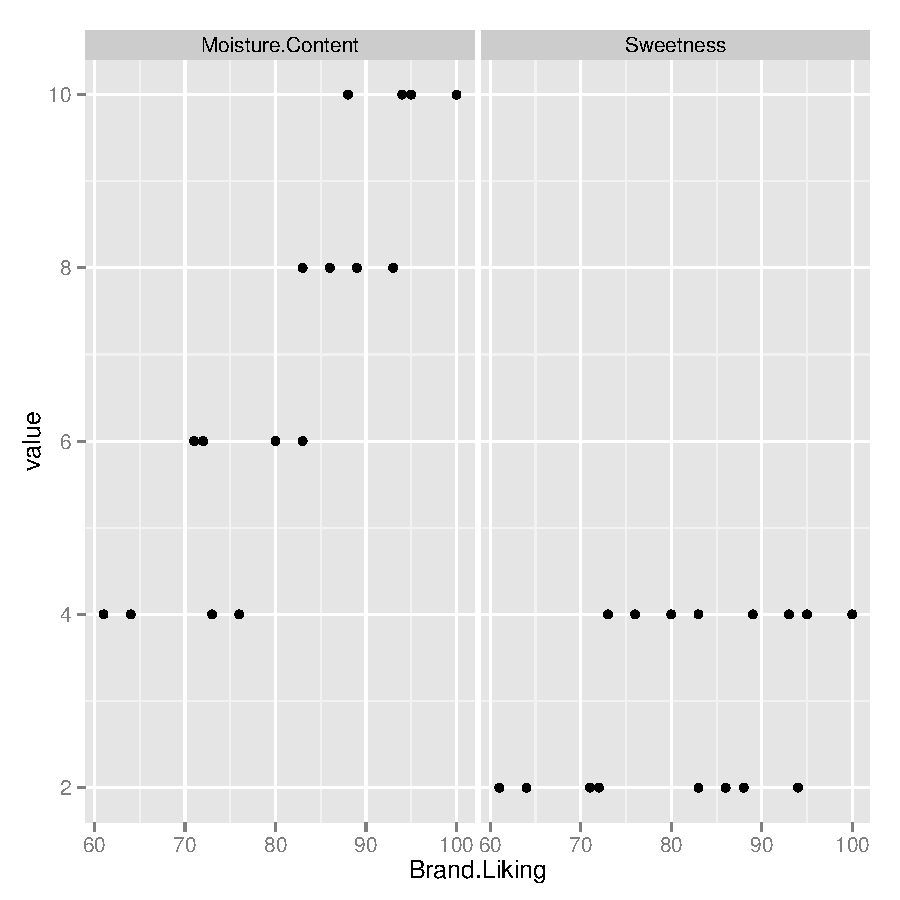
\includegraphics{Fig-scatterplot}

And now let's compute the correlation matrix:

\begin{Schunk}
\begin{Sinput}
> cor(BrandPreference)
\end{Sinput}
\begin{Soutput}
                 Brand.Liking Moisture.Content Sweetness
Brand.Liking        1.0000000        0.8923929 0.3945807
Moisture.Content    0.8923929        1.0000000 0.0000000
Sweetness           0.3945807        0.0000000 1.0000000
\end{Soutput}
\end{Schunk}

\item{} Now let's estimate the model $Y_i = b_0 + b_1X_{i1} + b_2X_{i2} + \epsilon{}_i$:
\begin{Schunk}
\begin{Sinput}
> fit <- lm(Brand.Liking~Moisture.Content+Sweetness,data=BrandPreference)
> fitsum <- summary(fit)
> fitsum
\end{Sinput}
\begin{Soutput}
Call:
lm(formula = Brand.Liking ~ Moisture.Content + Sweetness, data = BrandPreference)

Residuals:
   Min     1Q Median     3Q    Max 
-4.400 -1.762  0.025  1.587  4.200 

Coefficients:
                 Estimate Std. Error t value Pr(>|t|)    
(Intercept)       37.6500     2.9961  12.566 1.20e-08 ***
Moisture.Content   4.4250     0.3011  14.695 1.78e-09 ***
Sweetness          4.3750     0.6733   6.498 2.01e-05 ***
---
Signif. codes:  0 ‘***’ 0.001 ‘**’ 0.01 ‘*’ 0.05 ‘.’ 0.1 ‘ ’ 1

Residual standard error: 2.693 on 13 degrees of freedom
Multiple R-squared:  0.9521,	Adjusted R-squared:  0.9447 
F-statistic: 129.1 on 2 and 13 DF,  p-value: 2.658e-09
\end{Soutput}
\end{Schunk}

So, the estimated model is:
$$ Y_i = 37.65 + 4.425X_{i1} + 4.375X_{i2} $$

\item{} Now let's examine the residuals:

\begin{Schunk}
\begin{Sinput}
> boxplot(fit$residuals)
\end{Sinput}
\end{Schunk}
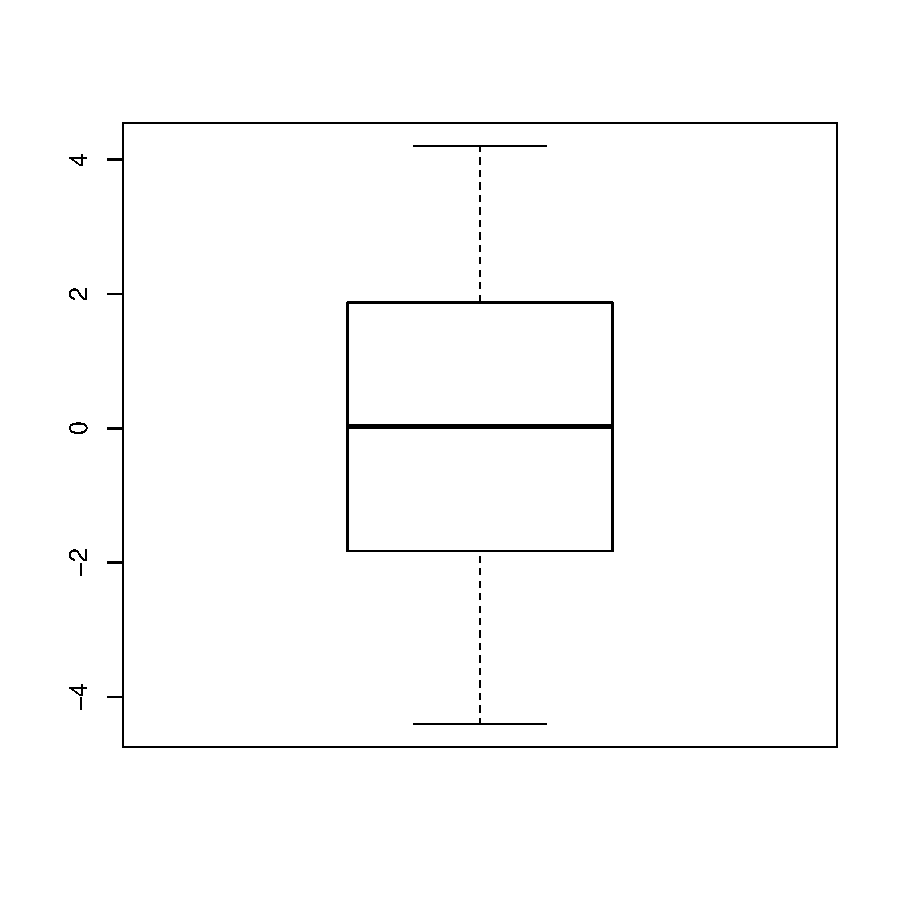
\includegraphics{Fig-resids}

This plot shows that the residuals are roughly normally distributed around 0.

\item{} Let's plot the residuals against $Y$, $X_1$, $X_2$ , and $X_1$ $X_2$:
 
\begin{Schunk}
\begin{Sinput}
> qplot(x=fit$residuals,
+       y=fit$model$Brand.Liking,
+       xlab="Residuals",
+       ylab="Brand Liking")
\end{Sinput}
\end{Schunk}
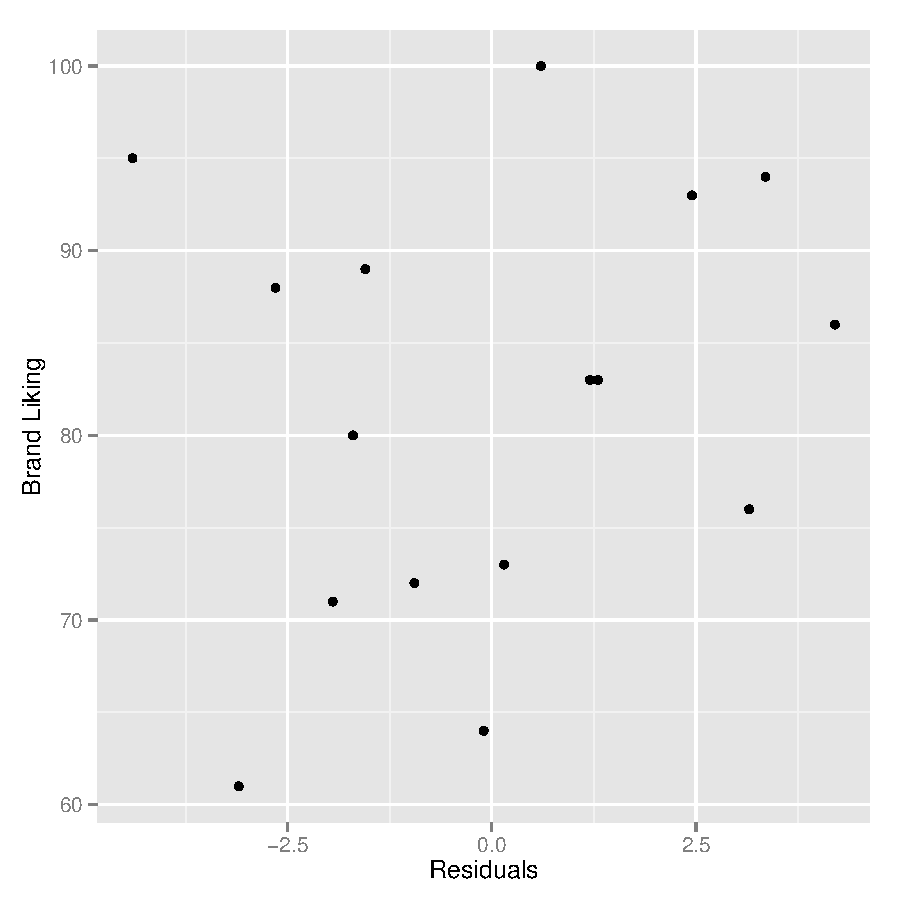
\includegraphics{Fig-moreplots}

\begin{Schunk}
\begin{Sinput}
> qplot(x=fit$residuals,
+       y=fit$model$Moisture.Content,
+       xlab="Residuals",
+       ylab="Moisture Content")
\end{Sinput}
\end{Schunk}
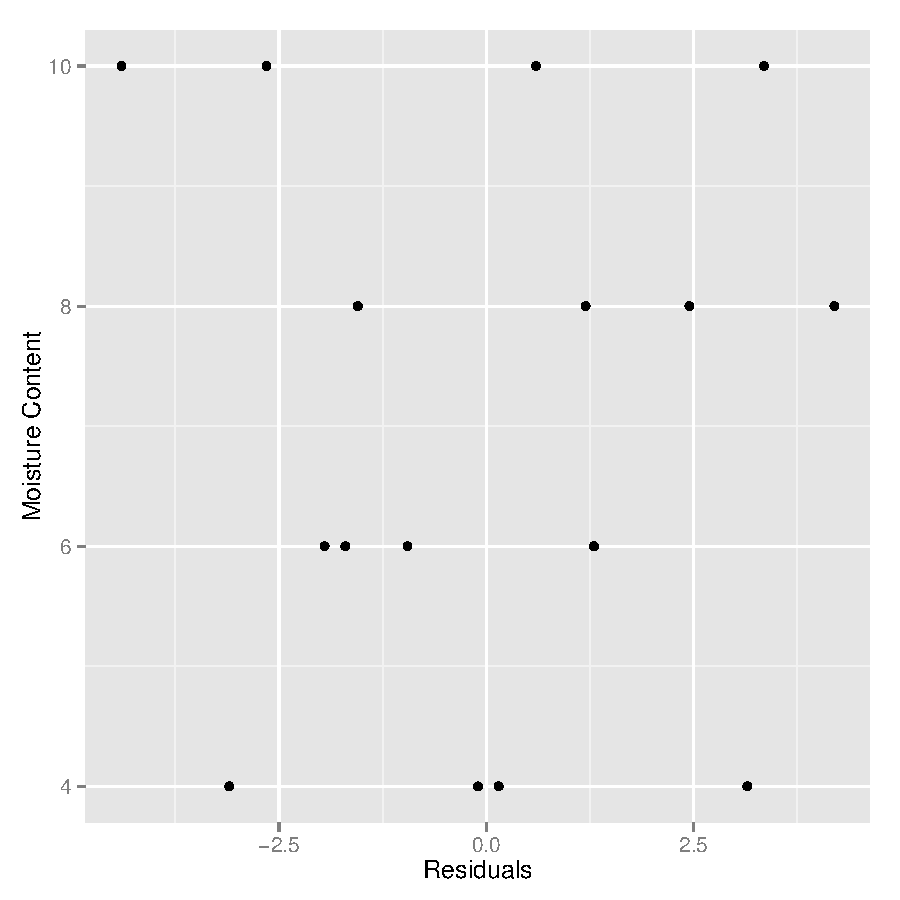
\includegraphics{Fig-moreplots2}

\begin{Schunk}
\begin{Sinput}
> qplot(x=fit$residuals,
+       y=fit$model$Sweetness,
+       xlab="Residuals",
+       ylab="Sweetness")
\end{Sinput}
\end{Schunk}
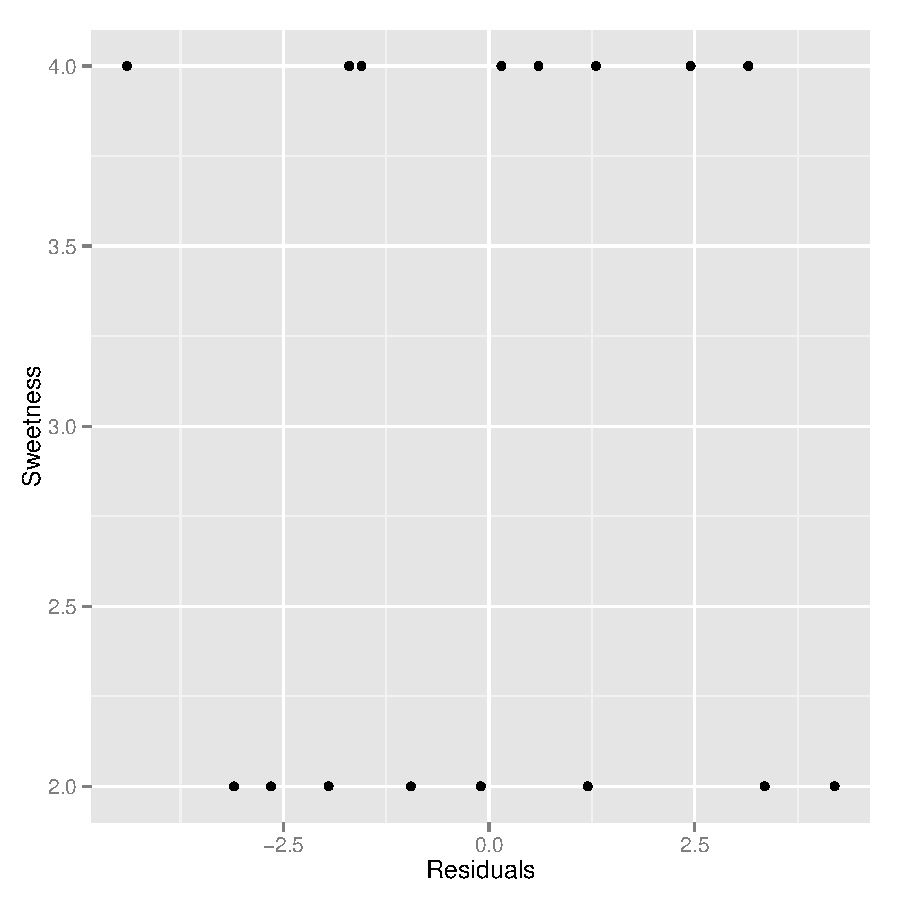
\includegraphics{Fig-moreplots3}

\begin{Schunk}
\begin{Sinput}
> qplot(x=fit$residuals,
+       y=fit$model$Moisture.Content*fit$model$Sweetness,
+       xlab="Residuals",ylab="Moisture Content times Sweetness")
\end{Sinput}
\end{Schunk}
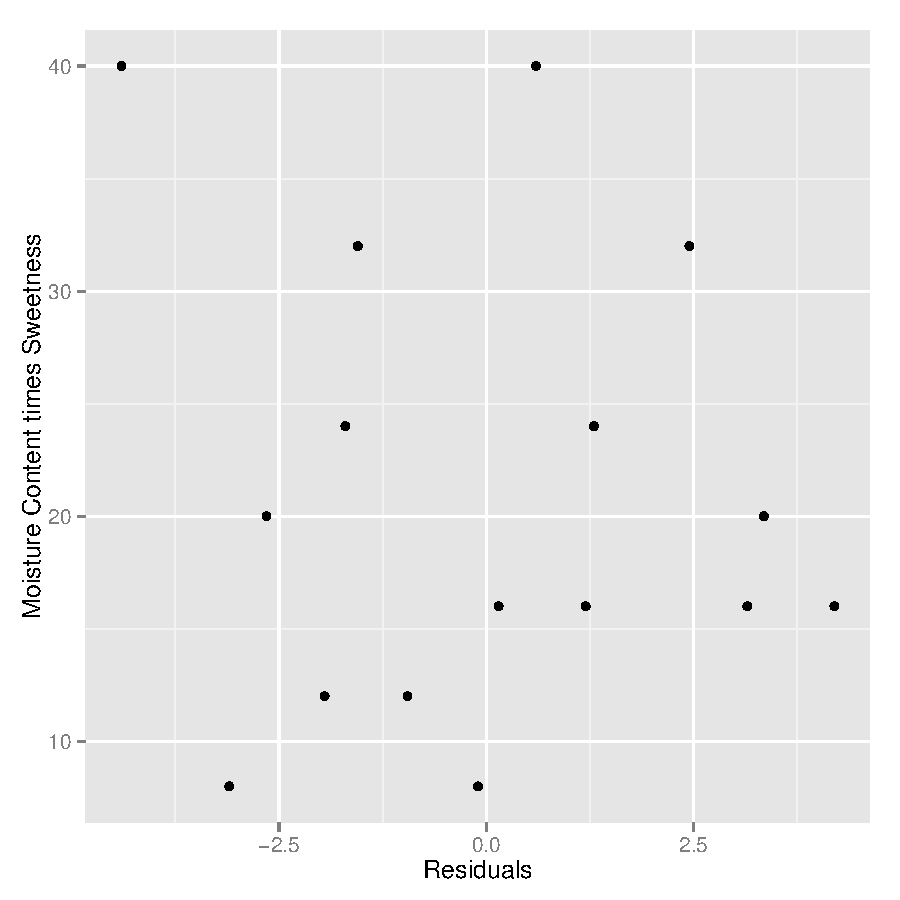
\includegraphics{Fig-moreplots4}

\begin{Schunk}
\begin{Sinput}
> qplot(sample=fit$residuals,
+       stat="qq",
+       main="Normal Probability Plot for Model Residuals")
\end{Sinput}
\end{Schunk}
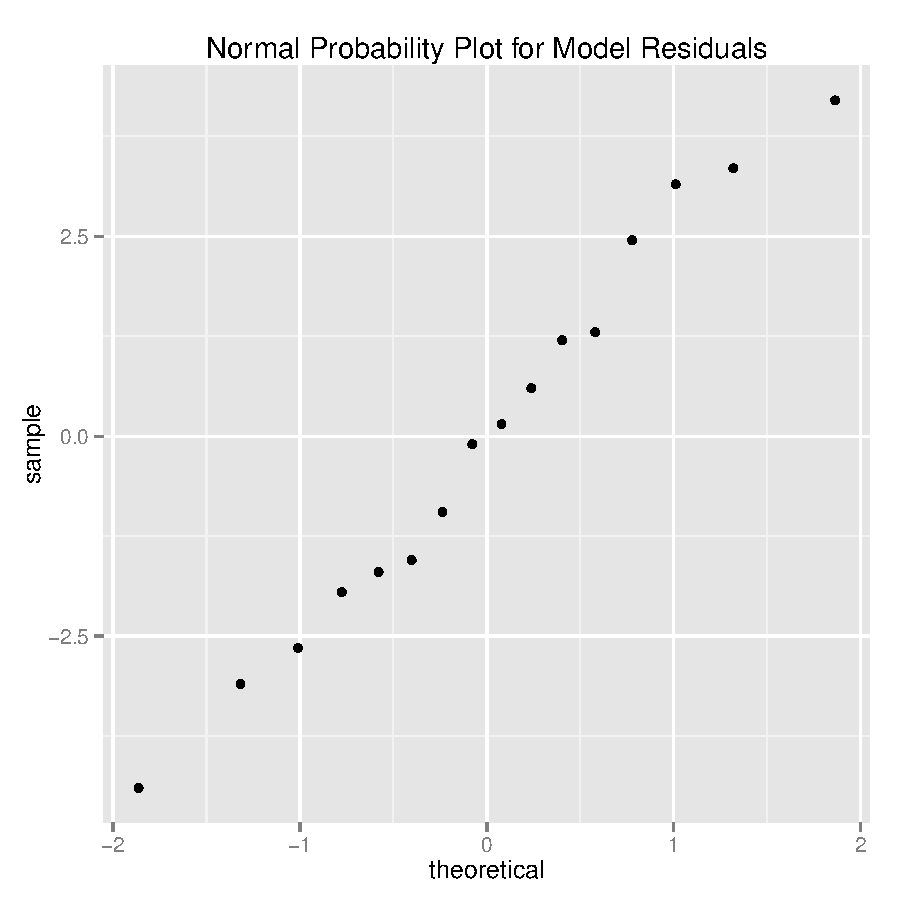
\includegraphics{Fig-moreplots5}

The plots indicate the the residuals are not only distributed normally, but are uncorrelated with either any of the predictors or the outcome. The model assumptions hold.

\item{} Let's perform the Breush-Pagan test for heteroskedasticity of the error terms

\begin{Schunk}
\begin{Sinput}
> require(lmtest)
> pb <- bptest(fit,studentize=F)
> pb
\end{Sinput}
\begin{Soutput}
	Breusch-Pagan test

data:  fit
BP = 1.0422, df = 2, p-value = 0.5939
\end{Soutput}
\end{Schunk}

Clearly, we cannot reject the null hypothesis that the model exhibits homoskedasticity.

\end{enumerate}

%-------------------------------------------
\section{7.3}
%--------------------------------------------

Refer to Brand Preference Problem 6.5:

\begin{enumerate}[a)]
\item{} Obtain the analysis of variance table that decomposes the regression sum of squares into extra sums of squares associated with $X_1$, and with $X_2$ , given $X_1$.
\item{} Test whether $X_2$ can be dropped from the regression model given that $X_1$ is retained. Use the $F^*$ test statistic and level of significance .01. State the alternatives, decision rule, and conclusion. What is the P-value of the test?
\end{enumerate}

\subsection{Answer:}

\begin{enumerate}[a)]
\item{} First we must fit the first order model:

\begin{Schunk}
\begin{Sinput}
> fo <- lm(Brand.Liking~Moisture.Content,data=BrandPreference)
> fosum <- summary(fo)
> fosum
\end{Sinput}
\begin{Soutput}
Call:
lm(formula = Brand.Liking ~ Moisture.Content, data = BrandPreference)

Residuals:
   Min     1Q Median     3Q    Max 
-7.475 -4.688 -0.100  4.638  7.525 

Coefficients:
                 Estimate Std. Error t value Pr(>|t|)    
(Intercept)        50.775      4.395  11.554 1.52e-08 ***
Moisture.Content    4.425      0.598   7.399 3.36e-06 ***
---
Signif. codes:  0 ‘***’ 0.001 ‘**’ 0.01 ‘*’ 0.05 ‘.’ 0.1 ‘ ’ 1

Residual standard error: 5.349 on 14 degrees of freedom
Multiple R-squared:  0.7964,	Adjusted R-squared:  0.7818 
F-statistic: 54.75 on 1 and 14 DF,  p-value: 3.356e-06
\end{Soutput}
\end{Schunk}

Now we can find $SSR(X_2|X_1)$:

\begin{Schunk}
\begin{Sinput}
> ssr_x2x1 <- deviance(fo) - deviance(fit)
> ssr_x2x1
\end{Sinput}
\begin{Soutput}
[1] 306.25
\end{Soutput}
\end{Schunk}

So, the extra sum of squares, $SSR(X_2|X_1) = 306.25$.

\item{} Now let's test to see if we can drop $X_2$ given $X_1$. The alternatives are as follows:

$$ H_0: \beta{}_3 = 0 $$
$$ H_a: \beta{}_3 \neq{} 0 $$

The decision rule is reject $H_0$ if:

$$ F^* > F(0.99,1,13) $$

Let's compute the test statistic and critical value:

\begin{Schunk}
\begin{Sinput}
> # test statistic
> F_star <- ((deviance(fo) - deviance(fit)) /
+   ((length(BrandPreference$Brand.Liking) - fosum$df[1]) - 
+      (length(BrandPreference$Brand.Liking) - fitsum$df[1]))) /
+   (deviance(fit)/(length(BrandPreference$Brand.Liking) - fitsum$df[1]))
> # critical value
> cv <- qf(0.99,1,length(BrandPreference$Brand.Liking)-fitsum$df[1])
> print(paste0("F^star is ",F_star," and the critical value is ",cv,"."))
\end{Sinput}
\begin{Soutput}
[1] "F^star is 42.2189819724284 and the critical value is 9.07380572851566."
\end{Soutput}
\end{Schunk}

Clearly we reject $H_0$ and conclude that $X_2$ should remain in the model. Let's compute the p-value of the test statistic:

\begin{Schunk}
\begin{Sinput}
> pval <- 1 - pf(F_star,1,length(BrandPreference$Brand.Liking)-fitsum$df[1])
> print(paste0("The p-value for F^star is: ",pval))
\end{Sinput}
\begin{Soutput}
[1] "The p-value for F^star is: 2.01104739359081e-05"
\end{Soutput}
\end{Schunk}

\end{enumerate}

%-------------------------------------------
\section{7.12}
%--------------------------------------------

Refer to Brand Preference Problem 6.5: Calculate $R_{Y1}^2$, $R_{Y2}^2$, $R_{|2}^2$, $R_{Y1|2}^2$, $R_{Y2|1}^2$, and $R^2$. Explain what each coefficient measures and interpret your results.

\subsection{Answer:}

\begin{enumerate}[a)]

\item{} $R_{Y1}^2$:

\begin{Schunk}
\begin{Sinput}
> anovafit <- anova(fit)
> r2_y1 <- anovafit["Moisture.Content","Sum Sq"]/sum(anovafit$`Sum Sq`)
> r2_y1
\end{Sinput}
\begin{Soutput}
[1] 0.796365
\end{Soutput}
\end{Schunk}

\item{} $R_{Y2}^2$:

\begin{Schunk}
\begin{Sinput}
> r2_y2 <- anovafit["Sweetness","Sum Sq"]/sum(anovafit$`Sum Sq`)
> r2_y2
\end{Sinput}
\begin{Soutput}
[1] 0.155694
\end{Soutput}
\end{Schunk}

\item{} $R_{|2}^2$:

\item{} $R_{Y1|2}^2$:

\begin{Schunk}
\begin{Sinput}
> fo2 <- lm(Brand.Liking~Sweetness,data=BrandPreference)
> fosum2 <- summary(fo2)
> r2_y12 <- (deviance(fo2) - deviance(fit))/deviance(fo2)
> r2_y12
\end{Sinput}
\begin{Soutput}
[1] 0.9432184
\end{Soutput}
\end{Schunk}

\item{} $R_{Y2|1}^2$:

\begin{Schunk}
\begin{Sinput}
> r2_y21 <- (deviance(fo) - deviance(fit))/deviance(fo)
> r2_y21
\end{Sinput}
\begin{Soutput}
[1] 0.7645737
\end{Soutput}
\end{Schunk}

\item{} $R^2$:

\begin{Schunk}
\begin{Sinput}
> r2 <- fitsum$r.squared
> r2
\end{Sinput}
\begin{Soutput}
[1] 0.952059
\end{Soutput}
\end{Schunk}

\end{enumerate}

%-------------------------------------------
\section{7.24}
%--------------------------------------------

Refer to Brand Preference Problem 6.5:

\begin{enumerate}[a)]
\item{} Fit first-order simple linear regression model (2.1) for relating brand liking ($Y$) to moisture content ($X_1$). State the fitted regression function.
\item{} Compare the estimated regression coefficient for moisture content obtained in part (a) with the corresponding coefficient obtained in Problem 6.5b. What do you find?
\item{} Does $SSR(X_1)$ equal $SSR(X_1|X_2)$ here? If not, is the difference substantial?
\item{} Refer to the correlation matrix obtained in Problem 6.5a. What bearing does this have on your findings in parts (b) and (c)?
\end{enumerate}

\subsection{Answer:}

\begin{enumerate}[a)]
\item{} Let's first fit the first order model:

\begin{Schunk}
\begin{Sinput}
> fo <- lm(Brand.Liking~Moisture.Content,data=BrandPreference)
> fosum <- summary(fo)
> fosum
\end{Sinput}
\begin{Soutput}
Call:
lm(formula = Brand.Liking ~ Moisture.Content, data = BrandPreference)

Residuals:
   Min     1Q Median     3Q    Max 
-7.475 -4.688 -0.100  4.638  7.525 

Coefficients:
                 Estimate Std. Error t value Pr(>|t|)    
(Intercept)        50.775      4.395  11.554 1.52e-08 ***
Moisture.Content    4.425      0.598   7.399 3.36e-06 ***
---
Signif. codes:  0 ‘***’ 0.001 ‘**’ 0.01 ‘*’ 0.05 ‘.’ 0.1 ‘ ’ 1

Residual standard error: 5.349 on 14 degrees of freedom
Multiple R-squared:  0.7964,	Adjusted R-squared:  0.7818 
F-statistic: 54.75 on 1 and 14 DF,  p-value: 3.356e-06
\end{Soutput}
\end{Schunk}

The estimated function is:
$$ Y_i = 50.775 + 4.425X_{i1} $$

\item{} Let's compare the estimated models:

\begin{Schunk}
\begin{Sinput}
> # two predictor model
> fitsum
\end{Sinput}
\begin{Soutput}
Call:
lm(formula = Brand.Liking ~ Moisture.Content + Sweetness, data = BrandPreference)

Residuals:
   Min     1Q Median     3Q    Max 
-4.400 -1.762  0.025  1.587  4.200 

Coefficients:
                 Estimate Std. Error t value Pr(>|t|)    
(Intercept)       37.6500     2.9961  12.566 1.20e-08 ***
Moisture.Content   4.4250     0.3011  14.695 1.78e-09 ***
Sweetness          4.3750     0.6733   6.498 2.01e-05 ***
---
Signif. codes:  0 ‘***’ 0.001 ‘**’ 0.01 ‘*’ 0.05 ‘.’ 0.1 ‘ ’ 1

Residual standard error: 2.693 on 13 degrees of freedom
Multiple R-squared:  0.9521,	Adjusted R-squared:  0.9447 
F-statistic: 129.1 on 2 and 13 DF,  p-value: 2.658e-09
\end{Soutput}
\begin{Sinput}
> # one predictor model
> fosum
\end{Sinput}
\begin{Soutput}
Call:
lm(formula = Brand.Liking ~ Moisture.Content, data = BrandPreference)

Residuals:
   Min     1Q Median     3Q    Max 
-7.475 -4.688 -0.100  4.638  7.525 

Coefficients:
                 Estimate Std. Error t value Pr(>|t|)    
(Intercept)        50.775      4.395  11.554 1.52e-08 ***
Moisture.Content    4.425      0.598   7.399 3.36e-06 ***
---
Signif. codes:  0 ‘***’ 0.001 ‘**’ 0.01 ‘*’ 0.05 ‘.’ 0.1 ‘ ’ 1

Residual standard error: 5.349 on 14 degrees of freedom
Multiple R-squared:  0.7964,	Adjusted R-squared:  0.7818 
F-statistic: 54.75 on 1 and 14 DF,  p-value: 3.356e-06
\end{Soutput}
\end{Schunk}

We find that the coefficients are the same in both models for Sweetness.

\item{} Let's find $SSR(X_1|X_2)$ and $SSR(X_1)$:

\begin{Schunk}
\begin{Sinput}
> SSR_x1x2 <- deviance(fo2) - deviance(fit)
> SSR_x1 <- sum(anova(fo)$`Sum Sq`) - deviance(fo)
> print(paste0("SSR(X1|X2) is ",SSR_x1x2," and SSR(X1) is ",SSR_x1))
\end{Sinput}
\begin{Soutput}
[1] "SSR(X1|X2) is 1566.45 and SSR(X1) is 1566.45"
\end{Soutput}
\end{Schunk}

Clearly $SSR(X_1|X_2)$ and $SSR(X_1)$ are both the same.

\item{} As suggested by the correlation matrix, Moisture Content and Sweetness are uncorrelated, so we would expect the estimated coefficients from part (b) to be the same for both models. We would also expect the $SSR(X_1|X_2)$ to be the same as $SSR(X_1)$ since $X_1$ and $X_2$ are unrelated. The presence or absence of $X_2$ provides no information about $X_1$. The converse is also true.

\end{enumerate}

%-------------------------------------------
\section{7.28}
%--------------------------------------------

\begin{enumerate}[a]
\item{} Define each of the following exta sums of squares: (I) $SSR(X_5|X_1)$, (2) $SSR(X_3,X_4|X_1)$, (3) $SSR(X_4|X_1,X_2,X_3)$.
\item{} For a multiple regression model with five $X$ variables, what is the relevant exta sum of squares for testing whether or not $\beta{}_5 = 0$? whether or not $\beta{}_2 = \beta{}_4 = 0$?
\end{enumerate}

\subsection{Answer:}

\begin{enumerate}[a)]
\item{}
\begin{enumerate}[1)]
\item{} $$ SSR(X_5|X_1) = SSR(X_1,X_5) - SSR(X_1) $$
\item{} $$ SSR(X_3,X_5|X_1) = SSR(X_1,X_3,X_5) - SSR(X_1) $$
\item{} $$ SSR(X_4|X_1,X_2,X_3) = SSR(X_1,X_2,X_3,X_4) - SSR(X_1,X_2,X_3) $$
\end{enumerate}
\item{} The relevant sum of squares for whether or not $\beta{}_5 = 0$:
$$ SSR(X_5|X_1,X_2,X_3,X_4,X_5) $$
The relevant sum of squares for whether or not $\beta{}_2 = \beta{}_4 = O$:
$$ SSR(X_2,X_4|X_1,X_3,X_5) $$
\end{enumerate}

%-------------------------------------------
\section{7.29}
%--------------------------------------------

Show that:
\begin{enumerate}[a)]
\item{} $SSR(X_1,X_2,X_3,X_4) = SSR(X_1) + SSR(X_2,X_3|X_1) + SSR(X4|X_1,X_2,X_3)$.
\item{} $SSR(X_1,X_2,X_3,X_4) = SSR(X_2,X_3) + SSR(X_1|X_2,X_3) + SSR(X4|X_1,X_2,X_3)$.
\end{enumerate}

\subsection{Answer:}

\begin{enumerate}[a)]
\item{} $$ SSR(X_1) + SSR(X_2,X_3|X_1) + SSR(X4|X_1,X_2,X_3) $$
$$ = SSR(X_1) + SSR(X_1,X_2,X_3) - SSR(X_1) + SSR(X_1,X_2,X_3,X_4) - SSR(X_1,X_2,X_3) $$
$$ = SSR(X_1,X_2,X_3,X_4) $$
as required.
\item{} $$ SSR(X_2,X_3) + SSR(X_1|X_2,X_3) + SSR(X4|X_1,X_2,X_3) $$
$$ = SSR(X_2,X_3) + SSR(X_1,X_2,X_3) - SSR(X_2,X_3) + SSR(X_1,X_2,X_3,X_4) - SSR(X_1,X_2,X_3) $$
$$ = SSR(X_1,X_2,X_3,X_4) $$
as required.
\end{enumerate}

%-------------------------------------------
\section{7.30}
%--------------------------------------------

Refer to Brand Preference Problem 6.5:

\begin{enumerate}[a)]
\item{} Regress $Y$ on $X_2$ using simple linear regression model (2.1) and obtain the residuals.
\item{} Regress $X_1$ on $X_2$ using simple linear regression model (2.1) and obtain the residuals.
\item{} Calculate the coefficient of simple correlation between the two sets of residuals and show that it equals $R_{Y1|2}$.
\end{enumerate}

\subsection{Answer:}

\begin{enumerate}[a)]
\item{} We have already previously estimated this model, so we can obtain the residuals:

\begin{Schunk}
\begin{Sinput}
> res_fo2 <- residuals(fo2)
> print(res_fo2)
\end{Sinput}
\begin{Soutput}
      1       2       3       4       5       6       7       8       9      10 
-13.375 -13.125 -16.375 -10.125  -5.375  -6.125  -6.375  -3.125   5.625   2.875 
     11      12      13      14      15      16 
  8.625   6.875  10.625   8.875  16.625  13.875 
\end{Soutput}
\end{Schunk}

\item{} Now let's regress $X_1$ on $X_2$ and obtain the residuals:

\begin{Schunk}
\begin{Sinput}
> xonx <- lm(Moisture.Content~Sweetness,data=BrandPreference)
> res_xonx <- residuals(xonx)
> print(res_xonx)
\end{Sinput}
\begin{Soutput}
 1  2  3  4  5  6  7  8  9 10 11 12 13 14 15 16 
-3 -3 -3 -3 -1 -1 -1 -1  1  1  1  1  3  3  3  3 
\end{Soutput}
\end{Schunk}

\item{} The simple correlation coefficient between the residuals for the two models is:

\begin{Schunk}
\begin{Sinput}
> cor(x=res_fo2,y=res_xonx)
\end{Sinput}
\begin{Soutput}
[1] 0.9711943
\end{Soutput}
\end{Schunk}

Now let's show that is is roughly equal to $r_{Y1|2}$:

\begin{Schunk}
\begin{Sinput}
> r_y12 <- sqrt((deviance(fo2) - deviance(fit))/deviance(fo2))
> r_y12
\end{Sinput}
\begin{Soutput}
[1] 0.9711943
\end{Soutput}
\end{Schunk}

Which is clearly the same as the coefficient of simple correlation between the two sets of residuals.

\end{enumerate}

%-------------------------------------------
\section{8.11}
%--------------------------------------------

Refer to Brand Preference Problem 6.5:

\begin{enumerate}[a)]
\item{} Fit regression model (8.22).
\item{} Test whether or not the interaction term can be dropped from the model; use $\alpha{} = .05$. State the alternatives, decision rule, and conclusion.
\end{enumerate}

\subsection{Answer:}

\begin{enumerate}[a)]
\item{} Let's fit the model:

\begin{Schunk}
\begin{Sinput}
> wint <- lm(Brand.Liking~Moisture.Content+Sweetness+Moisture.Content*Sweetness,
+            data=BrandPreference)
> wint_sum <- summary(wint)
> wint_sum
\end{Sinput}
\begin{Soutput}
Call:
lm(formula = Brand.Liking ~ Moisture.Content + Sweetness + Moisture.Content * 
    Sweetness, data = BrandPreference)

Residuals:
   Min     1Q Median     3Q    Max 
-4.150 -1.488  0.125  1.700  3.700 

Coefficients:
                           Estimate Std. Error t value Pr(>|t|)    
(Intercept)                 27.1500     6.4648   4.200  0.00123 ** 
Moisture.Content             5.9250     0.8797   6.735 2.09e-05 ***
Sweetness                    7.8750     2.0444   3.852  0.00230 ** 
Moisture.Content:Sweetness  -0.5000     0.2782  -1.797  0.09749 .  
---
Signif. codes:  0 ‘***’ 0.001 ‘**’ 0.01 ‘*’ 0.05 ‘.’ 0.1 ‘ ’ 1

Residual standard error: 2.488 on 12 degrees of freedom
Multiple R-squared:  0.9622,	Adjusted R-squared:  0.9528 
F-statistic: 101.9 on 3 and 12 DF,  p-value: 8.379e-09
\end{Soutput}
\end{Schunk}

\item{} Now let's test and see if the interaction term can be removed from the model. The alternatives are as follows:

$$ H_0: \beta{}_4 = 0 $$
$$ H_a: \beta{}_4 \neq{} 0 $$

The decision rule is reject $H_0$ if:

$$ F^* > F(0.95,1,12) $$

Let's compute the test statistic and critical value:

\begin{Schunk}
\begin{Sinput}
> # test statistic
> F_star <- ((deviance(fit) - deviance(wint)) /
+   ((length(BrandPreference$Brand.Liking) - fitsum$df[1]) - 
+      (length(BrandPreference$Brand.Liking) - wint_sum$df[1]))) /
+   (deviance(wint)/(length(BrandPreference$Brand.Liking) - wint_sum$df[1]))
> # critical value
> cv <- qf(0.95,1,length(BrandPreference$Brand.Liking)-wint_sum$df[1])
> print(paste0("F^star is ",F_star," and the critical value is ",cv,"."))
\end{Sinput}
\begin{Soutput}
[1] "F^star is 3.23014804845221 and the critical value is 4.7472253467225."
\end{Soutput}
\end{Schunk}

Clearly we fail to reject $H_0$ and conclude that $X_1X_2$ should not remain in the model. Let's compute the p-value of the test statistic:

\begin{Schunk}
\begin{Sinput}
> pval <- 1 - pf(F_star,1,length(BrandPreference$Brand.Liking)-wint_sum$df[1])
> print(paste0("The p-value for F^star is: ",pval))
\end{Sinput}
\begin{Soutput}
[1] "The p-value for F^star is: 0.0974862454531731"
\end{Soutput}
\end{Schunk}

\end{enumerate}

%-------------------------------------------
\section{8.16}
%--------------------------------------------

Refer to Grade point average Problem 1.19. An assistant to the director of admissions conjectured that the predictive power of the model could be improved by adding information on whether the student had chosen a major field of concentration at the time the application was submitted. Assume that regression model (8.33) is appropriate, where $X_1$ is entrance test score and $X_2 = 1$ if student had indicated a major field of concentration at the time of application and 0 if the major field was undecided. 

\begin{enumerate}[a)]
\item{} Explain how each regression coefficient in model (8.33) is interpreted here.
\item{} Fit the regression model and state the estimated regression function.
\item{} Test whether the $X_2$ variable can be dropped from the regression model; use $\alpha{} = .01$. State the alternatives. decision rule. and conclusion.
\item{} Obtain the residuals for regression model (8.33) and plot them against $X_1X_2$. Is there any evidence in your plot that it would be helpful to include an interaction term in the model?
\end{enumerate}

\subsection{Answer:}

\begin{enumerate}[a)]
\item{} $\beta{}_1$ can be interpreted as the effect of a one unit increase in entrance test score - a one unit increase in entrance test score yeilds a $\beta{}_1$ unit increase in a student's first year GPA, on average. $\beta{}_2$ can be interpreted as the average difference in GPA points associated with students who stated thier major field at the time of application irrespective of entrance test score.
\item{} Fit the model:

\begin{Schunk}
\begin{Sinput}
> GPA <- read.table(file='8.16.txt',stringsAsFactors=F)
> names(GPA) <- c("GPA","Entrance.Test","Major.Indicated")
> gpafit <- lm(GPA~Entrance.Test+Major.Indicated,data=GPA)
> gpafit_sum <- summary(gpafit)
> gpafit_sum
\end{Sinput}
\begin{Soutput}
Call:
lm(formula = GPA ~ Entrance.Test + Major.Indicated, data = GPA)

Residuals:
     Min       1Q   Median       3Q      Max 
-2.70304 -0.35574  0.02541  0.45747  1.25037 

Coefficients:
                Estimate Std. Error t value Pr(>|t|)    
(Intercept)      2.19842    0.33886   6.488 2.18e-09 ***
Entrance.Test    0.03789    0.01285   2.949  0.00385 ** 
Major.Indicated -0.09430    0.11997  -0.786  0.43341    
---
Signif. codes:  0 ‘***’ 0.001 ‘**’ 0.01 ‘*’ 0.05 ‘.’ 0.1 ‘ ’ 1

Residual standard error: 0.6241 on 117 degrees of freedom
Multiple R-squared:  0.07749,	Adjusted R-squared:  0.06172 
F-statistic: 4.914 on 2 and 117 DF,  p-value: 0.008928
\end{Soutput}
\end{Schunk}

The estimated model is:
$$ Y_i = 2.19841928804895 + 0.0378939641261244X_{i1} + 0.0378939641261244X_{i2} $$

\item{} Now let's test and see if $X_2$ can be removed from the model. The alternatives are as follows:

$$ H_0: \beta{}_3 = 0 $$
$$ H_a: \beta{}_3 \neq{} 0 $$

The decision rule is reject $H_0$ if:

$$ F^* > F(0.99,1,117) $$

Let's compute the test statistic and critical value:

\begin{Schunk}
\begin{Sinput}
> # test statistic
> gpafo <- lm(GPA~Entrance.Test,data=GPA)
> gpafo_sum <- summary(gpafo)
> F_star <- ((deviance(gpafo) - deviance(gpafit)) /
+   ((length(GPA$GPA) - gpafo_sum$df[1]) - 
+      (length(GPA$GPA) - gpafit_sum$df[1]))) /
+   (deviance(gpafit)/(length(GPA$GPA) - gpafit_sum$df[1]))
> # critical value
> cv <- qf(0.99,1,length(GPA$GPA)-gpafit_sum$df[1])
> print(paste0("F^star is ",F_star," and the critical value is ",cv,"."))
\end{Sinput}
\begin{Soutput}
[1] "F^star is 0.617931372908239 and the critical value is 6.85656380811069."
\end{Soutput}
\end{Schunk}

Clearly we fail to reject $H_0$ and conclude that $X_2$ should not remain in the model. Let's compute the p-value of the test statistic:

\item{} Let's plot the residuals vs the variable $X_1X_2$:

\begin{Schunk}
\begin{Sinput}
> qplot(x=residuals(gpafit),
+       y=Entrance.Test*Major.Indicated,data=GPA,
+       xlab="Residuals",
+       ylab="Entrance Test Score times Indicator Variable for Major Declaration")
\end{Sinput}
\end{Schunk}
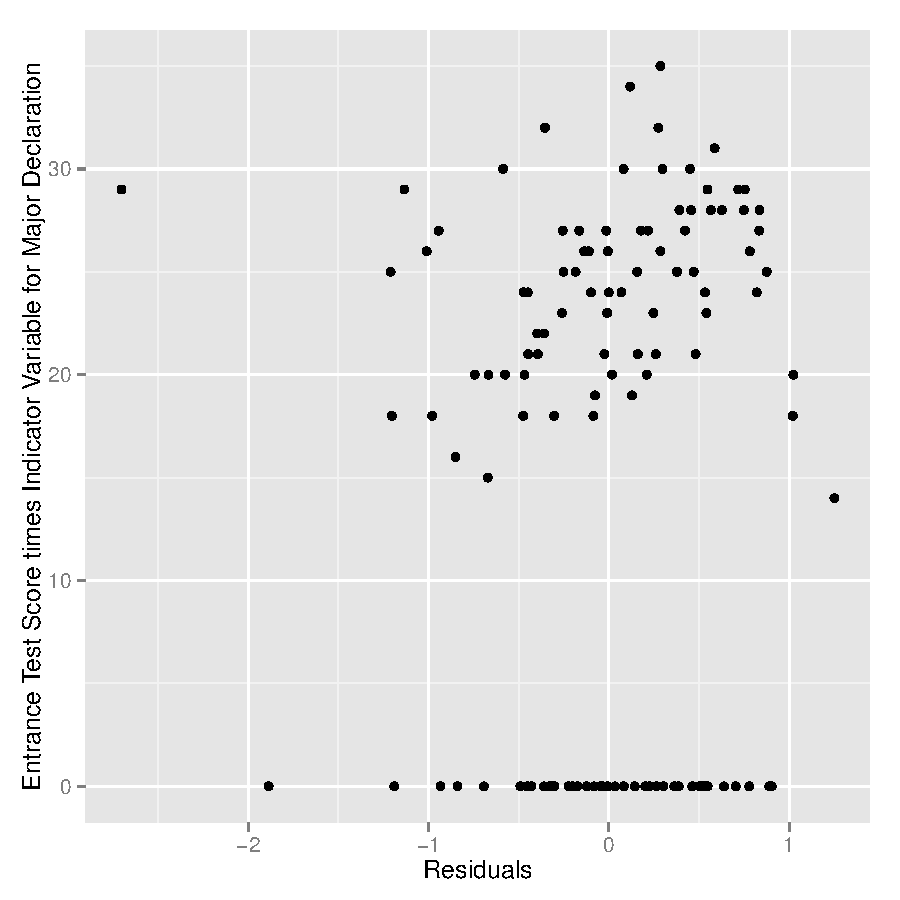
\includegraphics{Fig-moreresplots}

There appears to be a positive relationship between the residuals and $X_1X_2$ when $X_2 = 0$. It may be beneficial to include the term.

\end{enumerate}

%-------------------------------------------
\section{8.20}
%--------------------------------------------

Refer to Grade point average Problems 1.19 and 8.16:

\begin{enumerate}[a)]
\item{} Fit regression model (8.49) and state the estimated regression function.
\item{} Test whether the interaction term can be dropped from the model; use $\alpha{} = .05$. State the alternatives. decision rule, and conclusion. If the interaction term cannot be dropped from the model, describe the nature of the interaction effect.
\end{enumerate}

\subsection{Answer:}

\begin{enumerate}[a)]
\item{} Fit the model:

\begin{Schunk}
\begin{Sinput}
> intfit <- lm(GPA~Entrance.Test+Major.Indicated+Entrance.Test*Major.Indicated,
+              data=GPA)
> intfit_sum <- summary(intfit)
> intfit_sum
\end{Sinput}
\begin{Soutput}
Call:
lm(formula = GPA ~ Entrance.Test + Major.Indicated + Entrance.Test * 
    Major.Indicated, data = GPA)

Residuals:
     Min       1Q   Median       3Q      Max 
-2.80187 -0.31392  0.04451  0.44337  1.47544 

Coefficients:
                               Estimate Std. Error t value Pr(>|t|)    
(Intercept)                    3.226318   0.549428   5.872 4.18e-08 ***
Entrance.Test                 -0.002757   0.021405  -0.129   0.8977    
Major.Indicated               -1.649577   0.672197  -2.454   0.0156 *  
Entrance.Test:Major.Indicated  0.062245   0.026487   2.350   0.0205 *  
---
Signif. codes:  0 ‘***’ 0.001 ‘**’ 0.01 ‘*’ 0.05 ‘.’ 0.1 ‘ ’ 1

Residual standard error: 0.6124 on 116 degrees of freedom
Multiple R-squared:  0.1194,	Adjusted R-squared:  0.09664 
F-statistic: 5.244 on 3 and 116 DF,  p-value: 0.001982
\end{Soutput}
\end{Schunk}

The estimated model is:
$$ Y_i = 3.2263184991274 + -0.00275741710296684X_{i1} + -1.64957722409641X_{i2} + 0.0622446509862124X_{i1}X_{i2} $$

\item{} Test whether the interaction term is beneficial to the model:




\end{enumerate}

%-------------------------------------------
\section{8.42}
%--------------------------------------------

Refer to Market share data set in Appendix C.3. Company executives want to be able to predict market share of their product ($Y$) based on merchandise price ($X_1$), the gross Nielsen rating points ($X_1$, an index of the amount of advertising exposure that the product received); the presence or absence of a wholesale pricing discount ($X_3 = 1$ if discount present: otherwise $X_3 = 0$); the presence or absence of a package promotion during the period ($X_4 = 1$ if promotion present: otherwise $X_4 = 0$): and year ($X_5$). Code year as a nominal level variable and use 2000 as the reference year.

\begin{enumerate}[a)]
\item{} Fit a first-order regression model. Plot the residuals against the fitted values. How well does the first-order model appear to fit the data?
\item{} Re-fit the model in part (a). After adding all second-order terms involving only the quantitative predictors. Test whether or not all quadratic and interaction terms can be dropped from the regression model: use $\alpha = .05$. State the alternatives. decision rule, and conclusion.
\item{} In part (a), test whether advertising index ($X_2$) and year ($X_5$) can be dropped from the model; use $\alpha = .05$. State the alternatives, decision rule, and conclusion.
\end{enumerate}

\subsection{Answer:}

\begin{enumerate}[a)]
\item{} First, let's read in the data and recode the year variable into an indicator with a base of the year 2000:

\begin{Schunk}
\begin{Sinput}
> MarketShare <- read.table('MarketShare.txt',stringsAsFactors=F)
> names(MarketShare) <- c("id","Market.Share","Merchandise.Price","Nielson.Rating","Wholesale.Price.Discount","Package.Promotion","Month","Year")
> MarketShare$i1999 <- 1*(MarketShare$Year == 1999)
> MarketShare$i2001 <- 1*(MarketShare$Year == 2001) 
> MarketShare$i2002 <- 1*(MarketShare$Year == 2002)
\end{Sinput}
\end{Schunk}

\end{enumerate}


%-------------------------------------------
\section{System Information}
%--------------------------------------------

\begin{Schunk}
\begin{Sinput}
> sessionInfo();
\end{Sinput}
\begin{Soutput}
R version 3.0.2 (2013-09-25)
Platform: x86_64-pc-linux-gnu (64-bit)

locale:
 [1] LC_CTYPE=en_US.UTF-8 LC_NUMERIC=C         LC_TIME=C           
 [4] LC_COLLATE=C         LC_MONETARY=C        LC_MESSAGES=C       
 [7] LC_PAPER=C           LC_NAME=C            LC_ADDRESS=C        
[10] LC_TELEPHONE=C       LC_MEASUREMENT=C     LC_IDENTIFICATION=C 

attached base packages:
[1] stats     graphics  grDevices utils     datasets  methods   base     

other attached packages:
[1] lmtest_0.9-32   zoo_1.7-10      reshape2_1.2.2  ggplot2_0.9.3.1

loaded via a namespace (and not attached):
 [1] MASS_7.3-29        RColorBrewer_1.0-5 colorspace_1.2-4   dichromat_2.0-0   
 [5] digest_0.6.3       grid_3.0.2         gtable_0.1.2       labeling_0.2      
 [9] lattice_0.20-23    munsell_0.4.2      plyr_1.8           proto_0.3-10      
[13] scales_0.2.3       stringr_0.6.2      tools_3.0.2       
\end{Soutput}
\end{Schunk}

\end{document}
